\documentclass[12pt,letterpaper,titlepage,en-US]{article}

\usepackage{basicstyle}
\usepackage{report}
\usepackage{knit}
\usepackage{amsmath}
\usepackage{xcolor}
\usepackage{listings}
\usepackage{fancyvrb}
\usepackage{graphicx}
\definecolor{lbcolor}{rgb}{0.969, 0.969, 0.969} 
 \lstset{ 
    language=C++, % choose the language of the code
    basicstyle=\fontfamily{pcr}\selectfont\footnotesize\color{black},
    keywordstyle=\color{black}, % style for keywords
    numbers=none, % where to put the line-numbers
    numberstyle=\tiny, % the size of the fonts that are used for the line-numbers     
    backgroundcolor=\color{lbcolor},
    showspaces=false, % show spaces adding particular underscores
    showstringspaces=false, % underline spaces within strings
    showtabs=false, % show tabs within strings adding particular underscores
    frame=single, % adds a frame around the code
    tabsize=2, % sets default tabsize to 2 spaces
    rulesepcolor=\color{gray},
    rulecolor=\color{black},
    captionpos=b, % sets the caption-position to bottom
    breaklines=true, % sets automatic line breaking
    breakatwhitespace=false, 
}


\newcommand{\hmwkTitle}{Mini Project \#1}
\DTMsavetimestamp{DueDate}{2019-01-31T10:00:00-06:00}
\newcommand{\hmwkClass}{CS 6313.001}
\newcommand{\hmwkClassName}{Statistical Methods for Data Science}
\newcommand{\hmwkClassInstructor}{Instructor: Prof. Min Chen}
\newcommand{\hmwkAuthorName}{Shyam Patharla}
\newcommand{\hmwkAuthorNetID}{sxp178231}

\newcommand{\hmwkAuthorOneName}{Lizhong Zhang (lxz160730) : P1(ae), P2(bcde)}
\newcommand{\hmwkAuthorTwoName}{Hanlin He (hxh160630) : P1(bcd), P2(af)}



%
% Title Page
%

\title{
    \vspace{1in}
    \textmd{\textbf{\hmwkClassName \\\hmwkClass:\ \hmwkTitle }}\\
     \normalsize\vspace{0.1in}\small{Due\ on\ \DTMusedate{DueDate}\ at \DTMusetime{DueDate} }\\
    \vspace{0.1in}\large{\textit{\hmwkClassInstructor}}\\
    \vspace{0.5in}
\includegraphics[height=2.4em]{UTD_logo_BW}\\
    \vspace{2in}
    }



\author{\textbf{\hmwkAuthorName\ \footnotesize{(\hmwkAuthorNetID)}} \\ }
\date{}
\makeindex

\begin{document}
\maketitle

\pagenumbering{Roman}

\tableofcontents

\pagebreak
\pagenumbering{arabic}


\section{Answers}

\subsection{Analytically calculating the probability that the lifetime of the satellite will exceed 15 years}
Based on the conditions in the problem, we have:
\begin{equation}
f_{T}(t) = \begin{cases} 0.2 e^{-0.1t} - 0.2 e^{-0.2t}, 0 \leq x < \infty,\\ 0, \text{otherwise} \end{cases}
\end{equation}
where T is the random variable representing the lifetime of the satellite.

We can calculate the following using formulas

\begin{equation}
P(T > 15) =\int_{15}^\infty f(t) \diff t\\
     =\int_{15}^\infty (0.2 e^{-0.1t} - 0.2 e^{-0.2t})dt \\
     = 0.3965
\end{equation}


\subsection{Monte Carlo Simulation}

\subsubsection{Simulate a Draw of $X_{A}, X_{B}$ and T}
We first simulate $X_{A}.$ From inverse transform method, we have:
\begin{equation}
U = F(X_{A}) =1 - e^{\lambda X_{A}} (X_{A}>0) 
\end{equation}


\begin{equation}
X_{A} = F^{-1}(U)
\end{equation}
Solving for $X_{A}$ we get:
\begin{equation}
X_{A} = -10 ln(1-U)
\end{equation}


Therefore, to simulate a draw from the distribution of $X_{A}$, we can call \texttt{\textbf{runif()}} function in R as follow:

\begin{knitrout}
\definecolor{shadecolor}{rgb}{0.969, 0.969, 0.969}\color{fgcolor}
\begin{kframe}

\begin{verbatim}
> Xa = (-10) * 2.303 * log10(1 - runif(1)) 
> print(Xa)

## [1]  5.694788
\end{verbatim}
\end{kframe}
\end{knitrout}

Since $X_{B}$ also has the same distribution as $X_{A}$ (exponential distribution with the same mean lifetime of 10 years), we repeat the procedure we did with $X_{A}$:

\begin{knitrout}
\definecolor{shadecolor}{rgb}{0.969, 0.969, 0.969}\color{fgcolor}
\begin{kframe}

\begin{verbatim}
> Xb =(-10) * 2.303 * log10(1 - runif(1)) 
> print(Xb)

## [1] 2.024587
\end{verbatim}
\end{kframe}
\end{knitrout}

We know the lifetime of a satellite in any draw is the sum of the lifetimes of we get in draws of $X_{A}$ and $X_{B}$. Using the above draws to simulate a draw for T, we get:

\begin{knitrout}
\definecolor{shadecolor}{rgb}{0.969, 0.969, 0.969}\color{fgcolor}
\begin{kframe}

\begin{verbatim}
> Xa + Xb

## [1]7.719375
\end{verbatim}
\end{kframe}
\end{knitrout}


\subsubsection{Repeat Step (a) 10,000 times}
We simulate 10,000 draws of T repeating the procedure in (a). 
\begin{knitrout}
\definecolor{shadecolor}{rgb}{0.969, 0.969, 0.969}\color{fgcolor}
\begin{kframe}

\begin{verbatim}
> t <- replicate(10000, (-10) * (2.303) * log10(1 - runif(1)) +
                 (2.303) * log10(1 - runif(1)) * (-10))

\end{verbatim}
\end{kframe}
\end{knitrout}

We save our draw results in vector t.


\subsubsection{Make a histogram of the 10,000 draws using 'hist' function}
Since random variables $X_{A}$ and $X_{B}$ have the same exponential distribution with the same parameter $\lambda$, their sum Z = $X_{A} + X_{B}$ also has the same parameter $\lambda$=0.1.
We plot the histogram using the following command in R:
\begin{knitrout}
\definecolor{shadecolor}{rgb}{0.969, 0.969, 0.969}\color{fgcolor}
\begin{kframe}

\begin{verbatim}
> hist(x, probability = TRUE, col = gray(.9), main = "Satellite Lifetime")
> curve( dexp(x,0.1), add = T )
\end{verbatim}
\end{kframe}
\end{knitrout}

We also draw the curve function of the probability of T with $\lambda=0.1$.
\begin{center}
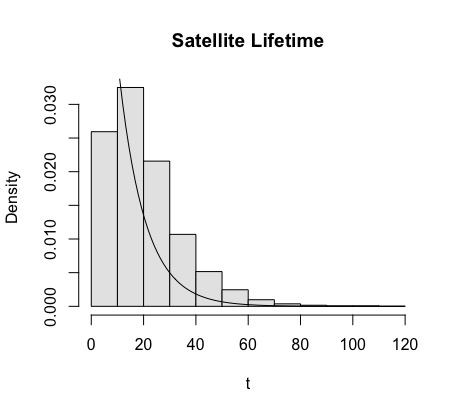
\includegraphics[scale=0.6]{hist.jpeg}
\end{center}

\subsubsection{Estimate E(T)}

We estimate the expected value of T using the following command:
\begin{knitrout}
\definecolor{shadecolor}{rgb}{0.969, 0.969, 0.969}\color{fgcolor}
\begin{kframe}
\begin{verbatim}
> mean(x)

## 19.9922
\end{verbatim}
\end{kframe}
\end{knitrout}
Analytical calculation gives us a value for E(T) of 15. We get a value of around 20 using Monte Carlo simulation.

\subsubsection{Estimate the probability that the satellite will last more than 15 years}
We run the following command to estimate P(T $>$ 15):
\begin{knitrout}
\definecolor{shadecolor}{rgb}{0.969, 0.969, 0.969}\color{fgcolor}
\begin{kframe}

\begin{verbatim}
> sum(x>15)/10000

## 0.5529
\end{verbatim}
\end{kframe}
\end{knitrout}
Analytical calculation gives us a value for P(T$>$15) of around 0.4. We get a value of 0.55 using Monte Carlo simulation.


\subsubsection{Taking 10,000 draws for 4 more times}

Using Monte Carlo simulation with 10,000 draws taken 4 times we get the results in \cref{1}.
\begin{table}[H]
\centering
\begin{tabular}{|c|c|c|}
\hline
Draw \#    &E(T)    & P(T$>$15) \\\hline
1 & 20.18618  &0.5636 \\\hline
2 & 20.10753  &0.5632\\\hline
3 &20.00512  &0.5580\\\hline
4 &19.95078  &0.5566\\\hline
\end{tabular}
\caption{4 Times 10000 Draws}\label{1}
\end{table}
The value of E(T) remains more or less stable around 20. The value of P(T$>$15) stabilises around 0.55


\subsection{Repeat part (e) 5 times with 1,000 and 100,000 draws instead of 10,000 }
Using Monte Carlo simulation with 1,000 draws taken 5 times we get the results in \cref{2}.
\begin{table}[H]
\centering
\begin{tabular}{|c|c|c|}
\hline
Draw \#    &E(T)    & P(T$>$15) \\\hline
1 &19.29913   &0.541\\\hline
2 &20.48910   &0.568\\\hline
3 &19.83506   &0.548\\\hline
4 &19.79278   &0.557\\\hline
5&20.22468   &0.543 \\\hline
\end{tabular}
\caption{Taking 1,000 Draws for 5 times}\label{2}
\end{table}
The value of E(T) remains more or less stable around 20. The value of P(T$>$15) stabilises around 0.5.

Using Monte Carlo simulation with 100,000 draws taken 5 times comes the results in \cref{3}
\begin{table}[H]
\centering
\begin{tabular}{|c|c|c|}
\hline
Draw \#    &E(T)    & P(T$>$15) \\\hline
1 &20.10833 &0.56098\\\hline
2& 19.95363 &0.55437\\\hline
3& 19.97778 &0.55673\\\hline
4& 20.02585 &0.55765\\\hline
5& 19.96851 &0.55651\\\hline

\end{tabular}
\caption{Taking 100,000 Draws for 5 times}\label{3}
\end{table}
The value of E(T) remains more or less stable around 20. The value of P(T$>$15) stabilises around 0.55. We get a greater stability in values compare with n=1000.



\subsection{Estimating the value of pi using Monte Carlo Simulation}
Consider a square of unit length with vertices at (0,0), (0,1), (1,0), and (1,1) and a circle circumscribed in it with centre at (0.5, 0.5) and a radius 0f 0.5 units. 
Let us look at the ratio of the area of the circle to the area of the square.

\begin{equation}
\dfrac{Area(Circle)}{Area(Square)} =\dfrac{ \pi* (0.5)^{2}}{ 1^{2}} = 0.25\pi
\end{equation}


Say we randomly choose a point inside the square. The probability that it falls inside the circle is $0.25\pi$. So we can see that:\\

$\pi$ = 4 * Probability (a random point chosen in the square falls inside the circle)\\

So we can randomly choose a point from the standard uniform distribution and see of it falls inside the circle, If we do this for 10,000 times and determine the probability above, we can approximate the value of pi.\\

To implement this, we first generate a random value from the standard uniform distribution for the value of x-coordinate. We repeat the same for the y coordinate. We then check if:

\begin{equation}
\sqrt{(x-0.5)^{2} + (y-0.5)^{2} }<= 0.5
\end{equation}  i.e. if the point lies inside the circle. We repeat this for 10,000 times. 

\begin{knitrout}
\definecolor{shadecolor}{rgb}{0.969, 0.969, 0.969}\color{fgcolor}
\begin{kframe}

\begin{verbatim}
> x = runif(10000)
> y = runif(10000)
> z = sqrt((x-0.5)^2 + (y-0.5)^2)
> sum(z<=0.5)/10000*4

## [1] 3.1464
\end{verbatim}
\end{kframe}
\end{knitrout}


\section{R Code}

\lstinputlisting{/users/psprao/downloads/stats/R-code/project1/Q1.R}
\lstinputlisting{/users/psprao/downloads/stats/R-code/project1/Q2.R}
\end{document}
